\documentclass{beamer}
\usepackage[utf8]{inputenc}

\usepackage{ulem}
\renewcommand<>{\sout}[1]{%
  \only#2{\beameroriginal{\sout}{#1}}%
  \invisible#2{#1}%
}

\usetheme{-bjeldbak/beamerthemebjeldbak}
\AtBeginSection[]{}

% \setbeameroption{show notes}
\setbeamertemplate{note page}[plain]
\setbeamerfont{note page}{size=\tiny}


\usepackage{animate}

\usepackage{graphicx,float,epstopdf,subcaption}
\graphicspath{{../report/results/}{../report/results/gen/}}

\usepackage{amsmath,amsfonts,bm,physics}
\usepackage[section]{algorithm}
\usepackage{algpseudocode}
\newcommand{\vect} [1] {\bm{#1}}
\newcommand{\mat} [1]{\mathbf{#1}}
\newcommand{\dra}{\dashrightarrow}
\newcommand{\dla}{\dashleftarrow}
\newcommand{\acc}{{\mkern 0.5mu\cdot\mkern 0.5mu}}

\usepackage{tikz}

\definecolor{colorA} {rgb} {0.1686, 0.5137, 0.7294}
\definecolor{colorB} {rgb} {0.9922, 0.6824, 0.3804}
\definecolor{colorC} {rgb} {0.4706, 0.6745, 0.4392}
\definecolor{colorD} {rgb} {0.8431, 0.0980, 0.1137}

\newcommand\theline[1]{%
    0.3 + 4.300298*(#1) - 4.615699*(#1)*(#1) + 1.752269*(#1)*(#1)*(#1) - 0.203497*(#1)*(#1)*(#1)*(#1)}


\title{Adaptive Meshes in Parallel}
\subtitle{(Parallel Adaptation of Orthotree Meshes)}
\subject{Parallel Adaptation of Orthotree Meshes}

\author{Matt Diesel \and Dr. Jie Li}
\institute{Cambridge University Engineering Department}
\date{Masters Project, 2017}

%\pgfdeclareimage[height=0.6cm]{cued-logo}{../report/Engineering.png}
%\logo{\usepgfimage{cued-logo}}

\begin{document}

\section{Intro}
\begin{frame}
    \titlepage
\end{frame}


\section{Motivation}
\begin{frame}
    \frametitle{Motivation}

    \begin{itemize}
        \item<1-3> Make things go faster
            \begin{itemize}
                \item<2> Drive down costs of testing
                \item<3> Allow computer optimisation
            \end{itemize}
        \item<4> Remove the limits of a single computer
    \end{itemize}
\end{frame}

\section{Prior Work}
\begin{frame}
    \frametitle{Optimising CFD}
    
    \begin{columns}
        \column{0.5\textwidth} 

            \begin{itemize}
                \item<1-> How do you make things go faster?
                    \begin{itemize}
                        \item<2> Better hardware 
                        \item<3> More hardware
                        \item<4-> Better software
                    \end{itemize}
            \end{itemize}

        \column{0.5\textwidth}

\only<5| handout:5>{
            \begin{tikzpicture}
                \input{gen/mesh-4-4-t0}
                \draw[domain=0:4,smooth,variable=\x,colorA, ultra thick] plot ({\x},
                    {\theline{4-\x}});
            \end{tikzpicture}

            1024 Cells
}

\only<6| handout:6>{
            \begin{tikzpicture}
                \input{gen/mesh-0-4-t0}
                \draw[domain=0:4,smooth,variable=\x,colorA, ultra thick] plot ({\x},
                    {\theline{4-\x}});
            \end{tikzpicture}

            169 Cells
}

\only<7| handout:7>{
            \begin{tikzpicture}
                \input{gen/mesh-0-4-t1}
                \draw[domain=0:4,smooth,variable=\x,colorA, ultra thick] plot ({\x},
                    {\theline{4-\x}});
            \end{tikzpicture}

            220 Cells.
}

\only<8| handout:8>{
    % Takes a long time to compile. 
    
\begin{animateinline}[autoplay,poster=last]{20}
    \multiframe{60}{n=0+1}{
        \begin{tikzpicture}
            \newcommand\topLayer{3}
            \node at (0,0) {};
            
            \ifnum 30>\n
                \begin{scope}[
                    yshift=2cm,every node/.append style={
                        yslant=0.5*\n/30,xslant=-\n/30},yslant=0.5*\n/30,xslant=-\n/30
                      ]
                    \fill[white,fill opacity=0] (0,0) rectangle (4,4);
                    % y = 0.3 + 6.189086*x - 6.682936*x^2 + 2.481516*x^3 - 0.2852701*x^4
                    \draw[domain=0:4,smooth,variable=\x,colorA, ultra thick] plot ({\x},
                        {\theline{4-\x}});
        
                    \input{gen/mesh-0-4-t1}
        
                \end{scope}
            \else
                \foreach \i in {\topLayer,...,0} {
                    \begin{scope}[
                        yshift=2cm+(1.2mm*(\topLayer-\i))*(\n-30),every node/.append style={
                            yslant=0.5,xslant=-1},yslant=0.5,xslant=-1
                          ]
                        \fill[white,fill opacity=0.5+0.4/30*(\n-30)] (0,0) rectangle (4,4);
                        % y = 0.3 + 6.189086*x - 6.682936*x^2 + 2.481516*x^3 - 0.2852701*x^4
                        \draw[domain=0:4,smooth,variable=\x,colorA, thick] plot ({\x},
                            {\theline{4-\x}});
            
                        \input{gen/layer-0-4-t1-l\i}
            
                        \draw[black,line width=2.5pt] (0,4) -- (0,0) -- (4,0);
                        \draw[black,line width=1.5pt] (0,4) -- (4,4) -- (4,0);
            
                    \end{scope}
                }
            \fi
        \end{tikzpicture}
    }
\end{animateinline}

}
    \end{columns}
\end{frame}


\section{Challenges}
\begin{frame}
    \frametitle{Challenges}

    \begin{columns}
        \column{0.5\textwidth} 

            \begin{itemize}
                \item<1> Gather \& Scatter
                \item<2> Balancing
                \item<3> ``Ghost'' cells
            \end{itemize}

        \column{0.5\textwidth}

\only<1>{
            \begin{tikzpicture}
                \input{gen/mesh-0-4-t1}
            \end{tikzpicture}
}

\only<2| handout:2>{
            \begin{tikzpicture}
                \begin{scope}[yshift=0,colorC,every node/.append style={fill=colorC!40}]
                    \input{gen/top}
                \end{scope}
                \begin{scope}[yshift=0,colorB,every node/.append style={fill=colorB!40}]
                    \input{gen/middle}
                \end{scope}
                \begin{scope}[yshift=0,colorD,every node/.append style={fill=colorD!40}]
                    \input{gen/bottom}
                \end{scope}
            \end{tikzpicture}
}

\only<3>{
            \begin{tikzpicture}
                \input{gen/mesh-0-4-t1}
            \end{tikzpicture}
}

    \end{columns}
\end{frame}


\section{Method}
\begin{frame}
    \frametitle{Method}

    \begin{columns}
        \column{0.5\textwidth} 

            \begin{itemize}
                \item<1> Tree Subsets
                \item<2> Distribution
                \item<3> Ghost \& Border Sets
                \item<4> Solving in parallel
                \item<5> Rebalancing
            \end{itemize}

        \column{0.5\textwidth}

            \begin{tikzpicture}
                \input{gen/mesh-0-4-t1}
            \end{tikzpicture}

    \end{columns}
\end{frame}

\begin{frame}
    \frametitle{Method - Distribution}

    \begin{columns}
        \column{0.5\textwidth} 

            Morton Curve

            ~

            \only<1| handout:1>{
                \begin{tikzpicture}
                    \begin{scope}[colorD,line width=0.6pt]
                        \input{../report/method/gen/tr-layer0}
                    \end{scope}
                    \begin{scope}[colorA]
                        \input{../report/method/gen/tr-mort-l0}
                    \end{scope}
                    \draw[line width=1.3pt] (0,0) rectangle (4,4); 
                \end{tikzpicture}
            }

            \only<2| handout:2>{
                \begin{tikzpicture}
                    \begin{scope}[colorD,line width=0.6pt]
                        \input{../report/method/gen/tr-layer1}
                    \end{scope}
                    \begin{scope}[line width=0.6pt]
                        \input{../report/method/gen/tr-layer0}
                    \end{scope}
                    \begin{scope}[colorA]
                        \input{../report/method/gen/tr-mort-l1}
                    \end{scope}
                    \draw[line width=1.3pt] (0,0) rectangle (4,4); 
                \end{tikzpicture}
            }

            \only<3| handout:3>{
                \begin{tikzpicture}
                    \begin{scope}[colorD,line width=0.6pt]
                        \input{../report/method/gen/tr-layer2}
                    \end{scope}
                    \begin{scope}[line width=0.6pt]
                        \input{../report/method/gen/tr-layer0}
                        \input{../report/method/gen/tr-layer1}
                    \end{scope}
                    \begin{scope}[colorA]
                        \input{../report/method/gen/tr-mort-l2}
                    \end{scope}
                    \draw[line width=1.3pt] (0,0) rectangle (4,4); 
                \end{tikzpicture}
            }

            \only<4-| handout:4->{
                \begin{tikzpicture}
                    \begin{scope}[colorD!50,line width=0.6pt]
                        \input{../report/method/gen/tr-layer2}
                    \end{scope}
                    \begin{scope}[line width=0.6pt,black!30]
                        \input{../report/method/gen/tr-layer0}
                        \input{../report/method/gen/tr-layer1}
                    \end{scope}
                    \begin{scope}[colorA!50]
                        \input{../report/method/gen/tr-mort-l2}
                    \end{scope}
                    \draw[line width=1.3pt,black!30] (0,0) rectangle (4,4); 
                \end{tikzpicture}
            }

        \column{0.5\textwidth}

            Rank Distribution

            ~

\only<1-3| handout:1-3>{
            \begin{tikzpicture}
                \begin{scope}[every node/.append style={color=black!30}]
                    \input{gen/mesh-0-4-t1}
                \end{scope}
            \end{tikzpicture}
}

\only<4| handout:4>{
            \begin{tikzpicture}
                \begin{scope}[yshift=0,colorC]
                    \input{gen/curve-mort0}
                \end{scope}
                \begin{scope}[yshift=0,colorD]
                    \input{gen/curve-mort1}
                \end{scope}
                \begin{scope}[yshift=0,colorB]
                    \input{gen/curve-mort2}
                \end{scope}
            \end{tikzpicture}
}

\only<5-| handout:5->{
            \begin{tikzpicture}
                \begin{scope}[yshift=0,colorC,every node/.append style={fill=colorC!40}]
                    \input{gen/mesh-mort0}
                \end{scope}
                \begin{scope}[yshift=0,colorD,every node/.append style={fill=colorD!40}]
                    \input{gen/mesh-mort1}
                \end{scope}
                \begin{scope}[yshift=0,colorB,every node/.append style={fill=colorB!40}]
                    \input{gen/mesh-mort2}
                \end{scope}
            \end{tikzpicture}
}

    \end{columns}
\end{frame}

\begin{frame}
    \frametitle{Method - Distribution}

    \begin{columns}
        \column{0.5\textwidth} 

            Hilbert Curve

            ~

            \only<1| handout:1>{
                \begin{tikzpicture}
                    \begin{scope}[colorD,line width=0.6pt]
                        \input{../report/method/gen/tr-layer0}
                    \end{scope}
                    \begin{scope}[colorA]
                        \input{../report/method/gen/tr-hilb-l0}
                    \end{scope}
                    \draw[line width=1.3pt] (0,0) rectangle (4,4); 
                \end{tikzpicture}
            }

            \only<2| handout:2>{
                \begin{tikzpicture}
                    \begin{scope}[colorD,line width=0.6pt]
                        \input{../report/method/gen/tr-layer1}
                    \end{scope}
                    \begin{scope}[line width=0.6pt]
                        \input{../report/method/gen/tr-layer0}
                    \end{scope}
                    \begin{scope}[colorA]
                        \input{../report/method/gen/tr-hilb-l1}
                    \end{scope}
                    \draw[line width=1.3pt] (0,0) rectangle (4,4); 
                \end{tikzpicture}
            }

            \only<3| handout:3>{
                \begin{tikzpicture}
                    \begin{scope}[colorD,line width=0.6pt]
                        \input{../report/method/gen/tr-layer2}
                    \end{scope}
                    \begin{scope}[line width=0.6pt]
                        \input{../report/method/gen/tr-layer0}
                        \input{../report/method/gen/tr-layer1}
                    \end{scope}
                    \begin{scope}[colorA]
                        \input{../report/method/gen/tr-hilb-l2}
                    \end{scope}
                    \draw[line width=1.3pt] (0,0) rectangle (4,4); 
                \end{tikzpicture}
            }

            \only<4-| handout:4->{
                \begin{tikzpicture}
                    \begin{scope}[colorD!50,line width=0.6pt]
                        \input{../report/method/gen/tr-layer2}
                    \end{scope}
                    \begin{scope}[line width=0.6pt,black!40]
                        \input{../report/method/gen/tr-layer0}
                        \input{../report/method/gen/tr-layer1}
                    \end{scope}
                    \begin{scope}[colorA!50]
                        \input{../report/method/gen/tr-hilb-l2}
                    \end{scope}
                    \draw[line width=1.3pt,black!40] (0,0) rectangle (4,4); 
                \end{tikzpicture}
            }

        \column{0.5\textwidth}

            Rank Distribution

            ~

\only<1-3| handout:1-3>{
            \begin{tikzpicture}[black!30]
                \input{gen/mesh-0-4-t1}
            \end{tikzpicture}
}

\only<4| handout:4>{
            \begin{tikzpicture}
                \begin{scope}[yshift=0,colorC]
                    \input{gen/curve-hilb0}
                \end{scope}
                \begin{scope}[yshift=0,colorD]
                    \input{gen/curve-hilb1}
                \end{scope}
                \begin{scope}[yshift=0,colorB]
                    \input{gen/curve-hilb2}
                \end{scope}
            \end{tikzpicture}
}

\only<5-| handout:5->{
            \begin{tikzpicture}
                \begin{scope}[yshift=0,colorC,every node/.append style={fill=colorC!40}]
                    \input{gen/mesh-hilb0}
                \end{scope}
                \begin{scope}[yshift=0,colorD,every node/.append style={fill=colorD!40}]
                    \input{gen/mesh-hilb1}
                \end{scope}
                \begin{scope}[yshift=0,colorB,every node/.append style={fill=colorB!40}]
                    \input{gen/mesh-hilb2}
                \end{scope}
            \end{tikzpicture}
}

    \end{columns}
\end{frame}


\begin{frame}
    \frametitle{Method - Ghosts}

    \begin{columns}
        \column{0.5\textwidth}
            Borders of Ranks$=1,2$

            ~

            \begin{tikzpicture}
                \begin{scope}[yshift=0,colorC!60,every node/.append style={fill=colorC!20}]
                    \input{gen/mesh-hilb0}
                \end{scope}
                \begin{scope}[yshift=0,colorD!60,every node/.append style={fill=colorD!20}]
                    \input{gen/mesh-hilb1}
                \end{scope}
                \begin{scope}[yshift=0,colorB!60,every node/.append style={fill=colorB!20}]
                    \input{gen/mesh-hilb2}
                \end{scope}
                \begin{scope}[yshift=0,colorD,every node/.append style={fill=colorD!60}]
                    \input{gen/borders-1}
                \end{scope}
                \begin{scope}[yshift=0,colorB,every node/.append style={fill=colorB!90}]
                    \input{gen/borders-2}
                \end{scope}
            \end{tikzpicture}
        \column{0.5\textwidth}
            Ghosts of Rank$=0$

            ~

            \begin{tikzpicture}
                \begin{scope}[yshift=0,colorC!60,every node/.append style={fill=colorC!20}]
                    \input{gen/mesh-hilb0}
                \end{scope}
                \begin{scope}[yshift=0,colorD!60,every node/.append style={fill=colorD!20}]
                    \input{gen/mesh-hilb1}
                \end{scope}
                \begin{scope}[yshift=0,colorB!60,every node/.append style={fill=colorB!20}]
                    \input{gen/mesh-hilb2}
                \end{scope}
                \begin{scope}[yshift=0,colorA,every node/.append style={fill=colorA!40}]
                    \input{gen/ghosts-0}
                \end{scope}
            \end{tikzpicture}
    \end{columns}
\end{frame}

\begin{frame}
    \frametitle{Method - Relaxation in Parallel}

    \begin{columns}
        \column{0.5\textwidth}
            Equation

            ~

            \begin{minipage}[c][4cm][c]{4cm}
            \begin{equation}
                \laplacian{\Phi}=\begin{cases}
                    -1 & \qq{if}\text{in circle} \\
                    0 & \qq{otherwise}
                \end{cases} \nonumber
            \end{equation}
            \end{minipage}

        \column{0.5\textwidth}
\only<1| handout:1>{
            Geometry

            ~

            \begin{minipage}[c][4cm][c]{4cm}
                \centering
                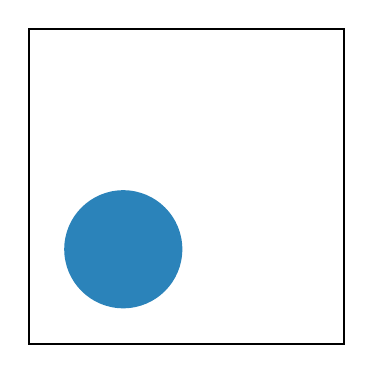
\begin{tikzpicture}
                    \draw[thick,black] (0,0) rectangle (4,4);
                    \node[thick,fill=colorA,inner sep=0, minimum size=1.5cm,circle] at (1.2,1.2) {};
                \end{tikzpicture}
            \end{minipage}
}

\only<2| handout:2>{
            Distribution (4 processes)

            ~

            \begin{tikzpicture}
                \begin{scope}[yshift=0,colorC,every node/.append style={fill=colorC!40}]
                    \input{gen/mesh-pois0}
                \end{scope}
                \begin{scope}[yshift=0,colorD,every node/.append style={fill=colorD!40}]
                    \input{gen/mesh-pois1}
                \end{scope}
                \begin{scope}[yshift=0,colorB,every node/.append style={fill=colorB!40}]
                    \input{gen/mesh-pois2}
                \end{scope}
                \begin{scope}[yshift=0,colorA,every node/.append style={fill=colorA!40}]
                    \input{gen/mesh-pois3}
                \end{scope}
            \end{tikzpicture}
}

\only<3| handout:3>{
            Solution

            ~

            \hspace{-1cm}
            \begin{minipage}[c][4cm][c]{4cm}
                \input{gen/pois-splot}
            \end{minipage}
}

    \end{columns}
\end{frame}


\begin{frame}
    \frametitle{Method - Rebalancing}

    \begin{columns}
        \column{0.5\textwidth}
            Circle at $(0.30,0.30)$

            ~

            \begin{tikzpicture}
                \begin{scope}[yshift=0,colorC,every node/.append style={fill=colorC!40}]
                    \input{gen/mesh-pois0}
                \end{scope}
                \begin{scope}[yshift=0,colorD,every node/.append style={fill=colorD!40}]
                    \input{gen/mesh-pois1}
                \end{scope}
                \begin{scope}[yshift=0,colorB,every node/.append style={fill=colorB!40}]
                    \input{gen/mesh-pois2}
                \end{scope}
                \begin{scope}[yshift=0,colorA,every node/.append style={fill=colorA!40}]
                    \input{gen/mesh-pois3}
                \end{scope}
            \end{tikzpicture}
        \column{0.5\textwidth}
            Circle at $(0.35,0.35)$

            ~

            \begin{tikzpicture}
                \begin{scope}[yshift=0,colorC,every node/.append style={fill=colorC!40}]
                    \input{gen/mesh-poism0}
                \end{scope}
                \begin{scope}[yshift=0,colorD,every node/.append style={fill=colorD!40}]
                    \input{gen/mesh-poism1}
                \end{scope}
                \begin{scope}[yshift=0,colorB,every node/.append style={fill=colorB!40}]
                    \input{gen/mesh-poism2}
                \end{scope}
                \begin{scope}[yshift=0,colorA,every node/.append style={fill=colorA!40}]
                    \input{gen/mesh-poism3}
                \end{scope}
            \end{tikzpicture}
    \end{columns}
\end{frame}


\section{Future Work}
\begin{frame}
    \frametitle{Future Work}
    \begin{columns}
        \column{0.5\textwidth}
            \begin{itemize}
                \item<1> Initial Distribution in Parallel
                \item<2> Refinement Propagation across Process Boundaries
            \end{itemize}
        \column{0.5\textwidth}
            ~

            ~

            \begin{tikzpicture}
                \begin{scope}[yshift=0,colorC,every node/.append style={fill=colorC!40}]
                    \input{gen/mesh-poism0}
                \end{scope}
                \begin{scope}[yshift=0,colorD,every node/.append style={fill=colorD!40}]
                    \input{gen/mesh-poism1}
                \end{scope}
                \begin{scope}[yshift=0,colorB,every node/.append style={fill=colorB!40}]
                    \input{gen/mesh-poism2}
                \end{scope}
                \begin{scope}[yshift=0,colorA,every node/.append style={fill=colorA!40}]
                    \input{gen/mesh-poism3}
                \end{scope}
            \end{tikzpicture}
    \end{columns}
\end{frame}

\section{Conclusions}
\begin{frame}
    \frametitle{Conclusions}

    \begin{itemize}
        \item<1> I developed a library to work with trees in parallel
        \item<2> The Hilbert curve is a good method for distribution.
        \item<3> It's possible to minimise the interprocess communication by maintaining equivalent ghost sets for process boundaries. 
        \item<4> It works, for a simple test case.
        \item<5> There are ways to do everything in parallel.
    \end{itemize}
\end{frame}

\end{document}
